\chapter{Software Architecture}\label{ch:architecture}

This chapter bridges the theoretical methodology and the practical implementation of our novelty detection system. 
We first present an overview of the software architecture, illustrating the end-to-end data flow from raw DNA sequences to patient-level anomaly scores. 
Then, we detail the primary algorithmic optimizations and engineering strategies implemented to ensure that the mismatch string kernel and Nystr\"{o}m approximations are efficient and memory-conscious when processing large genomic datasets.

\section{System Architecture Overview}\label{sec:overview}

Before discussing the specific algorithmic optimizations, it is useful to outline the high-level architecture and data flow of our system. 
The pipeline is designed modularly, separating data ingestion, feature extraction, kernel computation and model training into distinct stages.

\begin{figure}[htbp]
    \centering
    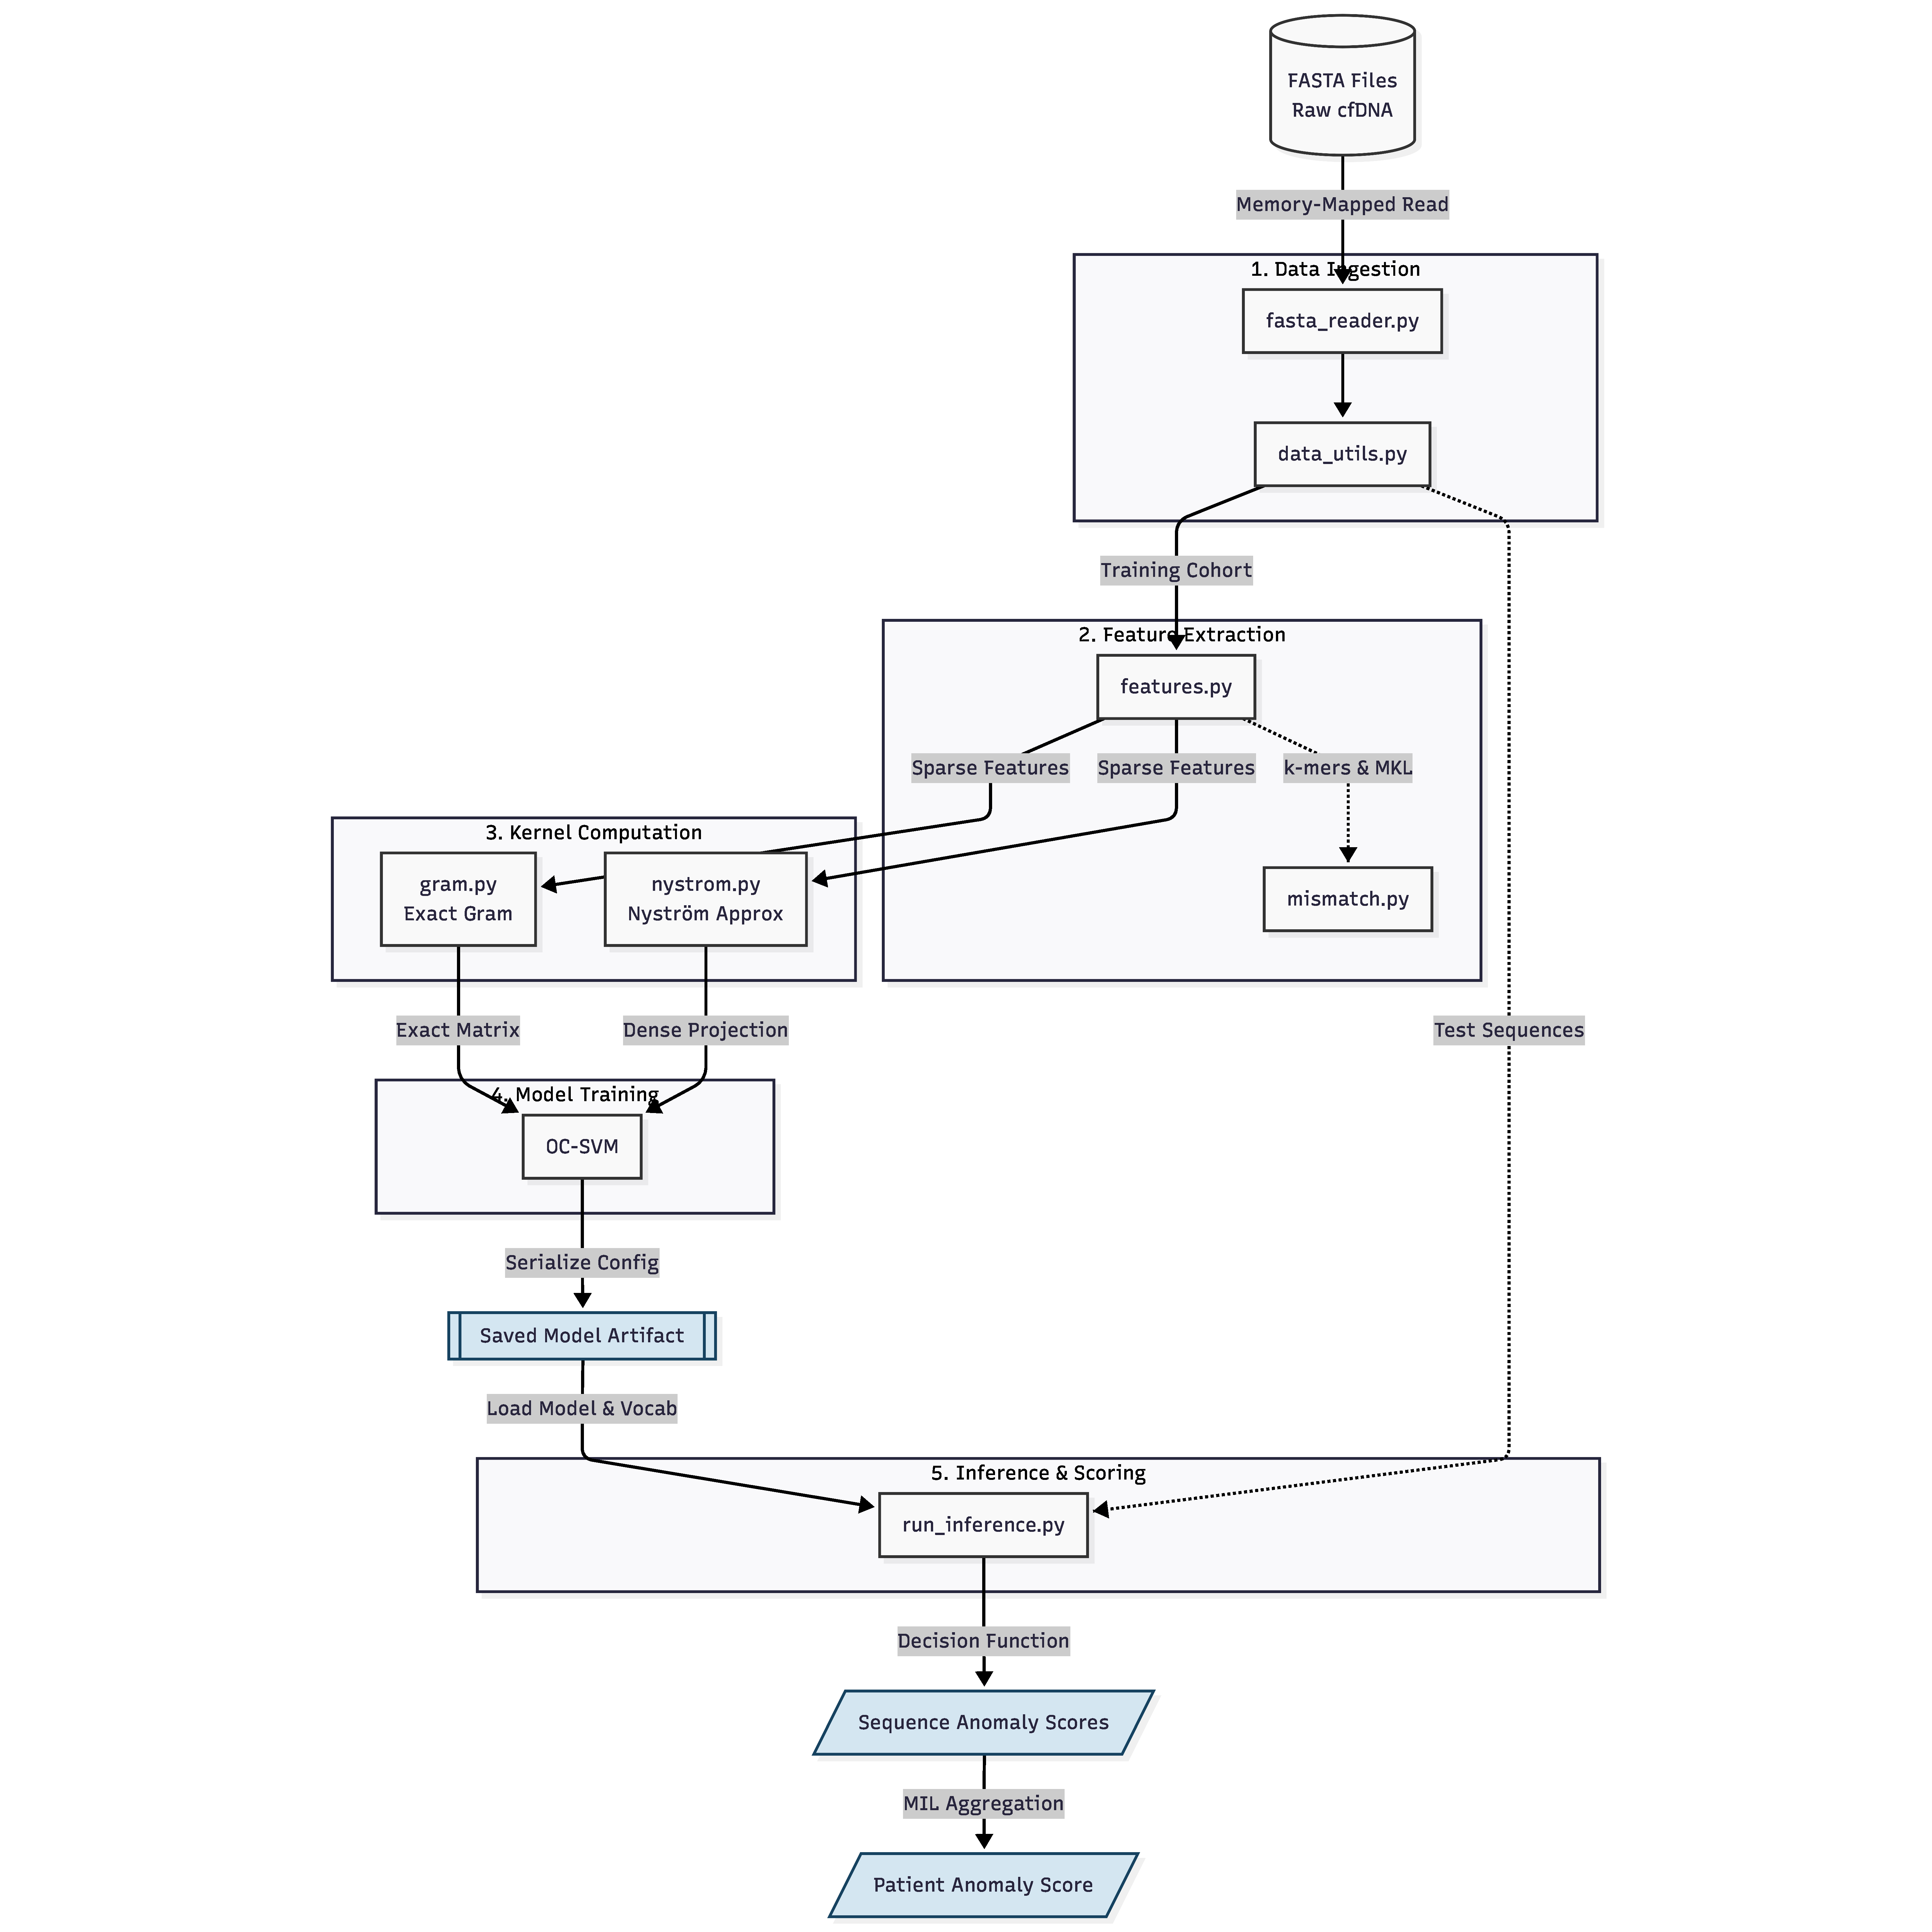
\includegraphics[width=\textwidth]{img/pipeline.pdf}
    \caption{High-level overview of the novelty detection pipeline, illustrating data flow from raw FASTA reads to anomaly scores.}
    \label{fig:pipeline}
\end{figure}

\subsection{Data Ingestion and Sampling}
The pipeline begins by parsing raw DNA fragments from \texttt{.fasta} files. Given the sheer volume of reads generated by sequencing, we utilize memory-mapped file reading (\texttt{fasta\_reader.py}) to allow fast, random-access lookups without loading the entire dataset into memory. 
A patient cohort is then loaded and a subset of fragments from healthy individuals is sampled to form the training set (\texttt{data\_utils.py}).

\subsection{Feature Extraction}
The raw DNA sequences are transformed into numerical representations. For a given sequence, we extract all overlapping substrings of length $k$ ($k$-mers) and generate their $m$-mismatch neighborhoods (\texttt{mismatch.py}). 
Because varying the length $k$ captures different biological motifs, we utilize Multiple Kernel Learning (MKL). Features from different $k$-mer lengths are weighted and concatenated into a unified sparse representation (\texttt{features.py}).

\subsection{Kernel Computation}
Once the sparse features are extracted, the system computes the exact Gram matrix representing the pairwise similarities between all sequences in the training set (\texttt{gram.py}). 
This symmetric matrix is evaluated using the dot product of the weighted $k$-mer frequency vectors. 
Because computing an exact Gram matrix requires $O(N^2)$ time and memory, our pipeline also includes an optional Nystr\"{o}m approximation module (\texttt{nystrom.py}). 
The Nystr\"{o}m method projects the sparse counts into a low-dimensional dense space using a subset of ``landmark'' sequences, drastically reducing the complexity for massive datasets.

\subsection{Model Training}
Finally, the computed kernel (or the dense Nystr\"{o}m projection) is fed into a One-Class Support Vector Machine (OC-SVM) from the \texttt{scikit-learn} library. 
The model is trained exclusively on normal patient DNA to learn the boundary of healthy genetic fragments. 
Once fitted, the model, with its configuration (e.g., MKL weights, maximum $k$, and mismatch tolerance), is serialized and saved as an artifact (\texttt{train\_and\_save\_svm.py}).

\subsection{Inference and Anomaly Scoring}
During the inference phase, sequences from a new, unclassified patient are evaluated against the trained model. 
The new fragments undergo the identical feature extraction and kernel projection steps using the serialized configuration and vocabulary from the training phase. 
The OC-SVM then assigns a decision score to each fragment, measuring its distance from the learned decision boundary. 
By inverting this decision value, we obtain a sequence-level anomaly score where higher values indicate a stronger deviation from the baseline of healthy cfDNA. 
These individual scores can then be aggregated to produce a comprehensive anomaly score for the entire patient.

\section{Algorithmic Optimisations}\label{sec:optimisations}

\subsection{Sparse Feature Representation}\label{sec:sparse}
For large $k$-mer lengths and small mismatch tolerances $m$, the feature vectors extracted from DNA sequences are extremely sparse. The vast majority of the $|\Sigma|^k$ possible $k$-mers never appear in a given sequence. Storing these representations as dense matrices would quickly exceed available memory constraints for datasets containing tens of thousands of sequences.

To address this, our implementation heavily relies on the \texttt{scipy.sparse} module. 
During feature extraction, observed $k$-mer frequencies (or distance-weighted scores) are accumulated in Coordinate list (COO) format---maintaining separate arrays for row indices, column indices, and values. This intermediate representation is fast to construct sequentially. 
Then, the COO data is converted into a Compressed Sparse Row (CSR) matrix, enabling fast matrix-vector dot products during the Gram matrix computation.

\begin{lstlisting}[language=Python, caption={Sparse matrix construction using COO format in \texttt{features.py}.}, label={lst:sparse}]
def _extract_chunk_weighted(chunk, chunk_offset, k, m, mismatch_decay, vocab):
    rows, cols, vals = [], [], []
    for local_idx, sequence in enumerate(chunk):
        # Generate raw k-mers and their mismatch neighborhoods
        # ...
        for col_idx, w in feature_weights.items():
            rows.append(chunk_offset + local_idx)
            cols.append(col_idx)
            vals.append(w)
            
    return rows, cols, vals

# Merge COO data from parallel chunks and construct CSR matrix
X = sp.csr_matrix(
    (np.array(all_vals), (np.array(all_rows), np.array(all_cols))),
    shape=(n_seqs, n_features),
)
\end{lstlisting}

\subsection{LRU-Cached Neighbourhood Generation}\label{sec:lru-cache}
Generating all possible $k$-mers within an $m$-mismatch distance is a combinatorial problem. 
Re-evaluating this neighborhood for every occurrence of a frequent $k$-mer introduces significant computational overhead. 
We alleviate this bottleneck by decorating our core neighborhood generation functions with Python's built-in \texttt{@lru\_cache}. 
This memoization technique ensures that once the mismatch neighborhood for a specific string is calculated, the result is cached in memory. Subsequent requests for the same $k$-mer bypass the combinatorial logic entirely, operating in $O(1)$ time.

\begin{lstlisting}[language=Python, caption={Memoized neighborhood generation in \texttt{mismatch.py}.}, label={lst:lru}]
from functools import lru_cache

@lru_cache(maxsize=100000)
def generate_weighted_mismatch_neighborhood(
    kmer: str, m: int = 1, alphabet = EPIGENETIC_ALPHABET
):
    # Combinatorial generation of neighboring k-mers
    # ...
    return tuple(neighbors.items())
\end{lstlisting}

\subsection{Pre-Enumerated Vocabulary}\label{sec:vocab}
Parallelizing the feature extraction process is non-trivial when the global vocabulary (the mapping of $k$-mers to column indices) is discovered dynamically. 
If multiple worker threads update a shared vocabulary simultaneously, it introduces race conditions and requires locking mechanisms, making parallelism difficult to achieve.

A solution consists of pre-enumerating the entire vocabulary of $|\Sigma|^k$ possible $k$-mers deterministically before extraction begins. 
By passing this fixed vocabulary down to the worker processes, each thread operates on an isolated chunk of sequences with no shared mutable state.

\begin{lstlisting}[language=Python, caption={Parallel feature extraction with pre-enumerated vocabulary in \texttt{features.py}.}, label={lst:vocab}]
# Pre-build full vocabulary mapping to column indices
vocab = build_full_vocabulary(k)

# Split sequences into chunks
chunk_boundaries = np.array_split(range(n_seqs), effective_jobs)
chunks = [(sequences[idx[0]:idx[-1]+1], idx[0]) for idx in chunk_boundaries]

# Parallel processing with no shared mutable state
results = Parallel(n_jobs=effective_jobs)(
    delayed(_extract_chunk_weighted)(
        chunk, offset, k, m, mismatch_decay, vocab
    )
    for chunk, offset in chunks
)
\end{lstlisting}

\subsection{Block-Partitioned Matrix Multiplication}\label{sec:block-parallel}
Computing the full Gram matrix $K = X \cdot X^T$ for a dataset of $N$ sequences requires an $N \times N$ dense matrix. For $N = 100,000$, this demands roughly 80 GB of RAM for a 64-bit float array. Performing this multiplication in a single operation can trigger out-of-memory errors or swapping problems.

Instead, we partition the Gram matrix into blocks of size $B \times B$ (typically $B=1500$). The dot product for each rectangular intersection $K[r_s:r_e, c_s:c_e] = X[r_s:r_e] \cdot X[c_s:c_e]^T$ is computed independently using \texttt{joblib}. 
This block-wise computation bounds peak memory consumption and allows maximum utilization of available CPU cores.

\begin{lstlisting}[language=Python, caption={Block-partitioned Gram matrix computation in \texttt{gram.py}.}, label={lst:block}]
def _compute_gram_block_pair(X_csr, r_start, r_end, c_start, c_end):
    # Compute block intersection
    block_val = X_csr[r_start:r_end].dot(X_csr[c_start:c_end].T).toarray()
    return r_start, r_end, c_start, c_end, block_val

# Generate task ranges
ranges = [(i, min(i + block_size, N)) for i in range(0, N, block_size)]
tasks = [(rs, re, cs, ce) for rs, re in ranges for cs, ce in ranges if cs >= rs]

# Execute parallel blocks
results = Parallel(n_jobs=n_inner_jobs, prefer="threads")(
    delayed(_compute_gram_block_pair)(X_k, rs, re, cs, ce)
    for rs, re, cs, ce in tasks
)
\end{lstlisting}